\documentclass[12pt]{article}

%%%%%%%%%%%%%%%%%%%%%%%%%%%%%%%  Packages  %%%%%%%%%%%%%
\usepackage{amsmath} 
\usepackage{mathtools}
\usepackage{physics}
\usepackage{amssymb}
\usepackage{mathptmx}
\usepackage{array}

%%%%%%%%% FIGurES %%%%%%%%%%%%%%%%%%%%%%%%
\usepackage{textcomp}
\usepackage{graphicx}
\usepackage{caption} 
\usepackage{subcaption}
\usepackage{scrextend}
\usepackage{pgfgantt}
\usepackage{rotating}
\usepackage{subcaption}
\usepackage{scrextend}
\usepackage{float}
%\graphicspath{ {figures/} }
\usepackage{hyperref}
\hypersetup{colorlinks=true, citecolor=blue, linkcolor=blue}
\renewcommand{\equationautorefname}{Eq.}%
\renewcommand{\figureautorefname}{Fig.}%

%%%%%%%%%%%% LaNgUaGe %%%%%%%%%%%%%%%%%%
\usepackage[latin1]{inputenc}
\usepackage{verbatim}
\usepackage{natbib}

%%%%%%%%%%%%%%%%%% Custom maths shortcuts %%%%%%%%%
\newcommand{\ident}{\[ \mathds{1} \]}

\renewcommand{\vec}[1]{\mathbf{#1}}
\newcommand{\squeezeup}{\vspace{-2.5mm}}
\newcommand{\rtwo}{\sqrt{2}}
%\DeclarePairedDelimiter\abs{\lvert}{\rvert}%
%\newcommand{\ket}[1]{\left| #1 \right\rangle}
%\newcommand{\bra}[1]{\left\langle #1 \right|}

\usepackage{qcircuit}
\usepackage{pdflscape}
\usepackage{afterpage}
\usepackage{wrapfig}
\usepackage[a4paper]{geometry}
\usepackage{multicol}

%%%%%%%%%%%%%%%%%%%%%%%%%%%%%%%%%%%%%%%%%%%%%%%%%%%%%%%%%
\newgeometry{left=0.8in,right=0.8in,top=1in,bottom=1in}
%%%%%%%%%%%%%%%%%%%%%%%%% EnD oF pAcKaGeS %%%%%%%%%%%%%%%%

\begin{document} %WOOP WOOP!
% Title page 

    \title{Quantum Circuits for the Schur Transform}
    \author{Oliver Thomas \\[0.5em] \\ Quantum Engineering CDT \\ University of Bristol}
    \date{\today}
    \maketitle

%%%%%%%%%%%%%%%%%%%%%%%%%%%%%%%%%%%%

\section{Introduction}

Universal distortion-free entanglement concentration \cite{blume2014streaming}, preparing highly symmetrized states for boson sampling  \cite{moylett2018quantum}, quantum data compression \cite{plesch2010efficient} and many other quantum information tasks \cite{harrow2005applications} can take advantage of an efficient implementation of the Schur transform. We look at existing algorithms for implementing the Schur transform and aim to produce a minimal gate quantum circuit which in principle could be used to implement the Schur transform on a small number of qubits in the near future \cite{kirby2017practical}.

There are two distinct ways of performing the Schur transform on n qubits, it can either be built up from coupling all n qubits together in a single iteration which we call the spatial multiplexed approach (as it acts on all qubits at once). The other approach is a streaming scheme which performs Clebsch-Gordan (CG) transforms on each of the n qubits one at a time which we call the temporal multiplexed approach (as it couples in one qubit at a time).  

This report is structured as follows, the Schur transform is introduced and we construct a quantum circuit numerically using the Givens rotation method \cite{li2013decomposition}. We comment on the scalability of this method and compare it to the analytical streaming procedure suggested in \cite{bacon2006efficient}. 

\section{The Schur Transform}

The Schur transform maps computation basis states to a Schur basis, in the qubit case this corresponds to performing a Clebsch-Gordan transform using the rules for addition of angular momentum. There are different ways of defining a Schur basis but here we choose to use angular momentum which is the natural choice for qubits. The notation used throughout we will call this Schur basis the spin basis. The spin basis is defined in terms of a labeling of J (Total angular momentum values), M (z-axis projection of the angular momentum) and multiplicity values which we refer to as P.

The Schur basis vectors for two qubits are,

\begin{subequations}
\begin{align}
\begin{split}
&\ket{J=1, M=+1} = \ket{00} \\
&\ket{J=1, M=\;\;\;0} = \frac{1}{\sqrt{2}}(\ket{01} + \ket{10}) \\
&\ket{J=1, M=-1} = \ket{11} \\
\end{split}\\
\begin{split}
&\ket{J=0, M=\;\;\;0} = \frac{1}{\sqrt{2}}(\ket{01} - \ket{10})\\
\end{split}
\end{align}
\end{subequations}

We have suppressed the multiplicity label here for simplicity as there are no multiplicities in the two qubit case. The matrix for the transform which takes the computational basis to the spin basis is,

\begin{align}
\begin{bmatrix}
1 & 0 & 0 & 0 \\
0 & \frac{1}{\sqrt{2}} & \frac{1}{\sqrt{2}} & 0 \\
0 & 0 & 0 & 1 \\
0 & \frac{1}{\sqrt{2}} & -\frac{1}{\sqrt{2}} & 0 \\
\end{bmatrix}
\begin{bmatrix}
\ket{00} \\
\ket{01} \\
\ket{10} \\
\ket{11} \\ 
\end{bmatrix}
=
\begin{bmatrix}
\ket{00} \\
\frac{1}{\sqrt{2}}(\ket{01} + \ket{10}) \\
\ket{11} \\
\frac{1}{\sqrt{2}}(\ket{01} - \ket{10}) \\ 
\end{bmatrix}
=
\begin{bmatrix}
\ket{J=1, M=1} \\
\ket{J=1, M=0} \\
\ket{J=1, M=-1} \\
\ket{J=0, M=0} \\ 
\end{bmatrix}
\end{align}

This transform takes the computational basis state, $\ket{01}$ to a superposition of the singlet and triplet states, $\frac{1}{\sqrt{2}} (\ket{J=1, M=0} + \ket{J=0, M=0})$. 

The Schur basis vectors can be calculated for any n qubit couplings using the Glebsch-Gordan coefficients, here we have calculated up to 4 qubits. For more than two qubits multiplicities are introduced, multiplicities keep track of which subspace the system is in. The multiplicities, P are defined as $J'-J$ which is the new J value after the coupling of the spin minus the previous J value. The number of combinations for a given amount of 1s in a P string is the number of multiplicities for that J value.

The transform for three qubits contains 8 terms, the allowed J values are J=3/2 which contains 4 states and J=1/2 which contains 2 states. The J=1/2 subspace contains 2 multiplicities corresponding to the two possible routes to that coupling, either J=1 to J=1/2 (couple down) or J=0 to J=1/2 (couple up). The basis vectors are given in the appendix for completeness \autoref{eq:3cgcoeff}. There are multiple ways of writing the spin basis vectors, the traditional CG coefficients and also what we refer to as the phase encoding \autoref{eq:phaseencode}. The phase encoded transform matrix will have a different decomposition as the shape of the matrix is different to the regular encoding. 

The transform for four qubits contains 16 terms, J=2 contains 5 terms, J=1 contains 3 terms with 3 multiplicities and the J=0 contains 1 term with 2 multiplicities. The equations are given in \autoref{eq:4qubitcg}. In the J=1 subspace there are 3 acceptable bit strings containing a single one, 0001, 0010 and 0100. This means there are 3 multiplicities present. 

\subsection{Schur Transform Circuits}

After building the unitary matrices from the Schur basis vectors using the CG coefficients we now calculate the gate cost of implementing the unitaries for 2, 3 and 4 qubits. See online \cite{githubot561} for FORTRAN code which implements the Givens rotation method to give the $C^{n-1}U$ decomposition for each of the Schur transform unitaries. 

As two-qubit (entangling) gates, denoted here by $C-U$, are much more expensive to perform compared to single qubit gates, the cost of the circuits discussed here will all be given in terms of the number of two-qubit gates. The decomposition scheme for the n-qubit case is bounded by $2^{n-1}(2^n-1)$ $C^{n-1}U$ gates \cite{li2013decomposition}, where $C^{n-1}U$ is defined as a unitary acting on 1 qubit controlled on the other n-1 qubits. It is possible to calculate a optimal gate sequence however current classical algorithms are computationally expensive \cite{sridharan2010reduced}.When n is greater than 2, it is possible to reduce higher order control gates to single control gates, $C^nU \sim 5 C^{n-1}V$ where $U \& V$ are unitaries \cite{barenco1995elementary}.

The two qubit Schur transform can be implemented in a circuit which only contains two gates as \autoref{cir:vanilla2},

%%%%%%%%% circuit 1 
\begin{figure}[h]
\begin{align*}
\Qcircuit @C=0.5cm @R=0.7cm{
%1
&\lstick{\ket{S_1}} &\gate{H} &\ctrl{1} &\qw \\
%0
&\lstick{\ket{S_0}} &\ctrl{-1} &\targ &\qw \\
}
\end{align*}
\caption{Schur transform for 2 qubits}
\label{cir:vanilla2}
\end{figure}

For 3 qubits the decomposition upper bound is 28 $C^2U$ gates. This implies the maximum two-qubit gates needed would be 140 $CU$ gates. The decomposition of the 3 qubit CG transform was performed analytically and using the Givens rotation method for unitary decomposition into a gate sequence to check the code converged to the correct sequence. The matrix \autoref{eq:3qubitcg} can be expressed as a product of 19 $C^2U$ gates (control-control-unitaries) which is $\sim$80 $CU$ gates. 

For the 4 qubits the decomposition requires at most 120 $C^3U$ gates ($\sim 3000$ $CU$ gates). The 4 qubit Schur transform was decomposed into 72 $C^3U$ gates ($\sim 1800 CU$ gates). These decompositions are not optimal however there exist algorithms to further optimise gate sequences \cite{shende2006synthesis} but are computationally expensive and not investigated here. The majority of gates were CNOT or equivalent gates, the 2 qubit gate set contained 1 out of 2 gates were CNOTs, 3 qubits, 14 out of 19 were $C^2$NOTs and 4 qubits, 50 out of 72 were $C^3$-NOT gates. This suggests a different approach was needed.

\section{Streaming Scheme}

Entanglement purification is an example of a process which gains an advantage when using a streaming scheme \cite{blume2014streaming}. It is possible to optimally perform purification in a streaming setup which is an advantage as it allows for some of the purified resource to be distributed while purifying the rest continually. The advantage gained from streaming is that it can still be useful to only purify part of the resource. There exists a streaming scheme for the Schur transform, however it is not useful to only be able to  perform a partial Schur transform. This suggests there may be other equivalent or better methods for implementing the Schur transform.      

The streaming scheme \autoref{fig:stream}, where the $U_{CG}$ is the Clebsch-Gordan transform between the $J$ \& $M$ registers and the k-th qubit $\ket{i_k}$. The $U_{CG}$ block can be chosen so that it contains all of the gates for up to the n-th qubit meaning the same block can be repeated. The $U_{CG}$ block is built up from \autoref{fig:ucg},  

\begin{figure}[H]
\centering
\begin{subfigure}[H]{0.49\textwidth}
\centering
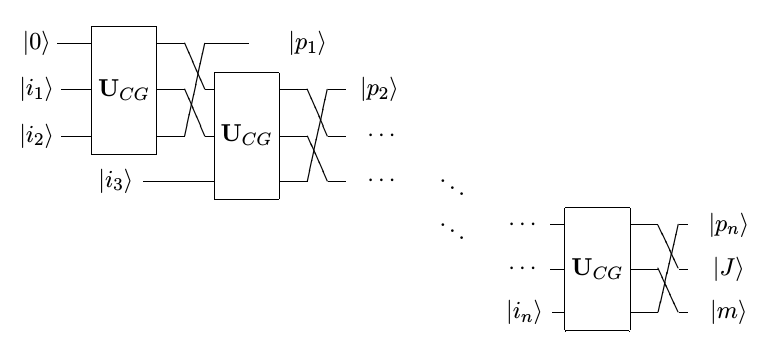
\includegraphics[width=0.9\textwidth]{schurcascade.png}
\caption{Streaming structure where the Schur transform is built up from consecutive Clebsch-Gordan transforms.}
\label{fig:stream}
\end{subfigure}
~
\begin{subfigure}[H]{0.49\textwidth}
\centering
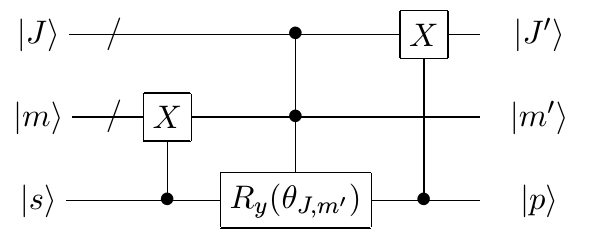
\includegraphics[width=0.9\textwidth]{genaddercirc.png}
\caption{$U_{CG}$ block, composed of a Qadder from qubit to M, controlled rotation on qubit conditional on J \& M' registers, Qadder transformed qubit to J.}
\label{fig:ucg}
\end{subfigure}
\caption{Streaming Schur Transform from \cite{bacon2006efficient}}  
\end{figure}

The controlled Rotation matrix \cite{bacon2006efficient}, $R_y(\theta_{J,m'})$ is the CG coefficients for coupling one qubit sequentially,

\begin{align}
\begin{split}
R_y(\theta_{J,m'})=
\begin{bmatrix}
\cos(\theta_{J,m'}) &-\sin(\theta_{J,m'}) \\
\sin(\theta_{J,m'}) & \cos(\theta_{J,m'}) \\
\end{bmatrix}
\end{split}
=
\begin{split}
\frac{1}{\sqrt{2J+1}}
\begin{bmatrix}
\sqrt{J+\frac{1}{2}+m'} &-\sqrt{J+\frac{1}{2}-m'} \\
\sqrt{J+\frac{1}{2}-m'} & \sqrt{J+\frac{1}{2}+m'} \\
\end{bmatrix}
\end{split}
\label{eq:rotmatrix}
\end{align}

Where primed variables mean the variable after the angular momentum addition, e.g. $J$ is the total angular momentum that the spin is coupling to, the whole system will have $J'$ total angular momentum after the coupling. $m$ is the z component of the system before and $m'$ is the total z component after the coupling.

To build this circuit the rotation matrix, $R_y(\theta_{J,m'})$ needs to be calculated using \autoref{eq:rotmatrix} (we calculate values in the appendix \autoref{eq:rvalues}) and the Qadder \autoref{fig:ucg} function to update the $\ket{m}$ and $\ket{J}$ registers is needed. Updating the registers can be implemented relatively simply using the coherent (registers are allowed to be in superpositions) equivalent of the digital adders and subtracters. The complexity now has been reduced to implementing the Clebsch-Gordan transform, $U_{CG}$.

\section{General Circuit for the Quantum Schur Transform}

In the section above we have investigated the cost of implementing directly the Clebsch-Gordan unitary matrix using a unitary gate decomposition scheme. We note that the majority, over half of the gates are CNOT or higher dimensional equivalents.

We now compare directly decomposing the Schur transform unitary to the streaming scheme above, the streaming method has the advantage of being modular and relatively easy to construct. Calculating and constructing the circuits (shown in \autoref{cir:tempmultistream}) was done by calculating the truth tables for each step. The quantum adder has already been studied and can be implemented using a reversible equivalent to a digital adder, \cite{draper2004logarithmic}. There are also other possibly more optimal schemes for very large registers which makes use of the quantum Fourier transform (QFT) \cite{draper2000addition}. These are outside the scope of this work as we are focusing on small numbers of qubits. The actual adder used here takes advantage of the fact the registers only ever change by $\pm1$ at each step \autoref{cir:genstreaming} . 

The general streaming circuit adds the value of the spin to be added $\ket{S}$ using the encoding $\ket{S} : \ket{0} \mapsto Spin = +\frac{1}{2}, \ket{1} \mapsto Spin = -\frac{1}{2}$ to the M register to calculate the M' register value. The CG transform gates are performed to generate P then the result is added to the J register to give the J' register value. The general circuit is shown in \autoref{cir:genstreaming}.

We note that it is possible to reduce the gate count of the general streaming scheme by changing the encoding. We remove the intermediate values which reduces both the number of qubits required and the gate count. This spatial multiplexing approach only stores the final output values of the $J$ \& $M$ registers whereas the streaming scheme stores all possible intermediate values. The scheme works by coupling in two qubits at a time as opposed to one (\autoref{cir:minspatialmult}, \autoref{cir:spatialmulti2}). 

\section{Discussion}

The majority of the gates are CNOT gates. This is mainly due to the re-ordering of the basis and is similar to the quantum Fourier transform (QFT). The QFT produces the output in reverse qubit order the actual number of gates required to do the transform is massively reduced. The overhead calculated here is due to the rearranging of the basis. This means that depending on what the transform is used the transform could be computed with less gates. For example, if the transform was only used to check if the state was in a particular J block but didn't need to know the specific M value the order afterwards wouldn't be as important reducing the CNOTs needed.

There is a lot of freedom in the choice of basis used. We have chosen to use Two's complement encoding for the registers. The encoding for the multiplicities remains consistent throughout although it is more complex. For the general circuits the encoding remains consistent throughout. In order to achieve the optimal number of gates for the Schur transform on a specific number of qubits the encoding is changed on a case by case basis. 

For large qubit coupling numbers the R matrix in the UCG tends to a Hadamard gate for the $\abs{M} < \abs{J}$ values of M. This means that depending on application of Schur transform and input states, it could be reasonable to approximate the transform when acting on highly symmetric states to just doing Hadamard gates.

We look at whether it is possible to achieve decrease in time by instead of coupling 1 qubit in at a time to the $J$ \& $M$ registers, to pairing each of the couplings up. This is the same as performing parts in parallel rather than sequentially. To investigate the problem we look at how the complexity of performing the Clebsch-Gordan transform scales moving from coupling a single qubit to an arbitrary $J \& M$ to coupling arbitrary $J \& M$ registers together. The pairing approach has a symmetry in the max range of $J \& M$ values will be the same within each pairing which will help simplify the problem compared to any arbitrary $J \& M$ values.

\section{Conclusion}

The streaming scheme uses temporal multiplexing to perform the Schur transform in polynomial time if a recursive streaming scheme is used \cite{bacon2007quantum}.


%%%%%%%%%%%%
\bibliographystyle{unsrt}
\bibliography{references}

\newpage
\appendix
\section{Appendix: Maths}

\subsection{3 Qubit transformation}

\begin{subequations}
\begin{align}
\intertext{ This is the J=3/2 block}
\begin{split}
&\ket{J=3/2, M=+3/2, P=000} = \ket{000} \\
&\ket{J=3/2, M=+1/2, P=000} = \sqrt{\frac{1}{3}}(\ket{001}+\ket{010}+\ket{100}) \\
&\ket{J=3/2, M=-1/2, P=000} = \sqrt{\frac{1}{3}}(\ket{110}+\ket{011}+\ket{101}) \\
&\ket{J=3/2, M=-3/2, P=000} = \ket{111} \\ 
\end{split} \\
\intertext{ This is the J=1/2 block from J=1, multiplicity zero}
\begin{split}
&\ket{J=1/2, M=+1/2, P=001} =+\sqrt{\frac{2}{3}}\ket{001} - \sqrt{\frac{1}{6}}(\ket{010}+\ket{100}) \\
&\ket{J=1/2, M=-1/2, P=001} =-\sqrt{\frac{2}{3}}\ket{110} + \sqrt{\frac{1}{6}}(\ket{011}+\ket{101}) \\ 
\end{split} \\
\intertext{ This is the J=1/2 block from J=0, multiplicity one}
\begin{split}
&\ket{J=1/2, M=+1/2, P=010} = \frac{1}{\rtwo} (\ket{010}-\ket{100})\\
&\ket{J=1/2, M=-1/2, P=010} = \frac{1}{\rtwo} (\ket{011}-\ket{101})\\
\end{split} 
\label{eq:3cgcoeff}
\end{align}
\end{subequations}

The CG transform for 3 qubits \autoref{eq:3qubitcg} can be rearranged to a block diagonal form which looks like it could be implemented in a circuit.
\begin{align}
\begin{bmatrix}
1 &0 &0 &0 &0 &0 &0 &0 \\
0 &\sqrt{\frac{2}{3}} &-\sqrt{\frac{1}{6}} &-\sqrt{\frac{1}{6}} &0 &0 &0 &0\\
0 &\sqrt{\frac{1}{3}} &\sqrt{\frac{1}{3}} &\sqrt{\frac{1}{3}} &0 &0 &0 &0\\
0 &0 &\frac{1}{\rtwo} &-\frac{1}{\rtwo} &0 &0 &0 &0 \\
0 &0 &0 &0 &\frac{1}{\rtwo} &-\frac{1}{\rtwo} &0 &0 \\
0 &0 &0 &0 &\sqrt{\frac{1}{3}} &\sqrt{\frac{1}{3}} &\sqrt{\frac{1}{3}} &0 \\
0 &0 &0 &0 &\sqrt{\frac{1}{6}} &\sqrt{\frac{1}{6}} &-\sqrt{\frac{2}{3}} &0 \\
0 &0 &0 &0 &0 &0 &0 &1 \\
\end{bmatrix}
\begin{bmatrix}
000 \\
001 \\
010 \\
100 \\
011 \\
101 \\
110 \\
111 \\
\end{bmatrix}
\end{align}

%%%%%%%%%%%%%%%%%%% 3 Qubits Phase encoding
\subsection{3 Qubit phase encoding}

\begin{subequations}
\begin{align}
\intertext{ This is the J=3/2 block}
\begin{split}
&\ket{J=3/2, M=+3/2, P=000} = \ket{000} \\
&\ket{J=3/2, M=+1/2, P=000} = \sqrt{\frac{1}{3}}(\ket{001}+\ket{010}+\ket{100}) \\
&\ket{J=3/2, M=-1/2, P=000} = \sqrt{\frac{1}{3}}(\ket{110}+\ket{011}+\ket{101}) \\
&\ket{J=3/2, M=-3/2, P=000} = \ket{111} \\ 
\end{split} \\
%\vspace{3pt} \nonumber\\
\intertext{ This is the J=1/2 block from J=1, multiplicity zero}
\begin{split}
&\ket{J=1/2, M=+1/2, P=001} = \frac{1}{\sqrt{3}} (\ket{001} + e^{2\pi i/3}\ket{100}+e^{4\pi i/3}\ket{010}) \\
&\ket{J=1/2, M=-1/2, P=001} =\frac{1}{\sqrt{3}} (\ket{011} + e^{2\pi i/3} \ket{101}+e^{4\pi i/3}\ket{110}) \\ 
\end{split} \\
%\vspace{3pt} \nonumber \\
\intertext{ This is the J=1/2 block from J=0, multiplicity one}
\begin{split}
&\ket{J=1/2, M=+1/2, P=010} = \frac{1}{\sqrt{3}} (\ket{001} + e^{4\pi i/3}\ket{100}+e^{2\pi i/3}\ket{010}) \\
&\ket{J=1/2, M=-1/2, P=010} =\frac{1}{\sqrt{3}} (\ket{011} + e^{4\pi i/3}\ket{101} +e^{2\pi i/3}\ket{110})\\
\end{split} 
\end{align}
\end{subequations}

The phase encoding matrix is given by,
% table pt 2 phase encoding

\begin{align}
\frac{1}{\sqrt{3}}
\begin{bmatrix}
\sqrt{3} &0 &0 &0 &0 &0 &0 &0 \\
0 &1 &1 &0 &1 &0 &0 &0 \\
0 &0 &0 &1 &0 &1 &1 &0\\
0 &0 &0 &0 &0 &0 &0 &\sqrt{3} \\
0 &e^{2\pi i/3} &e^{4\pi i/3} &0 &1 &0 &0 &0 \\
0 &0 &0 &e^{2\pi i/3} &0 &e^{4\pi i/3} &1 &0 \\
0 &e^{4\pi i/3} &e^{2\pi i/3} &0 &1 &0 &0 &0\\
0 &0 &0 &e^{4\pi i/3} &0 &e^{2\pi i/3} &1 &0 \\
\end{bmatrix}
\begin{bmatrix}
000 \\
001 \\
010 \\
011 \\
100 \\
101 \\
110 \\
111 \\
\end{bmatrix}
=
\begin{bmatrix}
\ket{J=3/2, M=3/2} \\
\ket{J=3/2, M=1/2} \\
\ket{J=3/2, M=-1/2} \\
\ket{J=3/2, M=-3/2} \\ 
\hline
\ket{J=1/2, M=1/2, P=0} \\
\ket{J=1/2, M=-1/2, P=0} \\
\hline
\ket{J=1/2, M=1/2, P=1} \\
\ket{J=1/2, M=-1/2, P=1} \\ 
\end{bmatrix}
%\end{align}
\label{eq:phaseencode}
\end{align}

Where this is a different form to the other basis for 3 qubits \autoref{eq:3qubitcg}.

\subsection{4 Qubit CG coefficients}
%%%%%%%%%%%%%%%%%%%%%%%%%%%%% 4 Qubit CG
\begin{subequations}
\begin{align}
%%%%%%%%%%%%%%%%%%%% J=2
\intertext{The J=2 block, P=0000, (J=1/2, J=1, J=3/2, J=2)}
\begin{split}
&\ket{J=2, M=+2, P=0000} = \ket{0000} \\
&\ket{J=2, M=+1, P=0000} = \frac{1}{2}(\ket{0001}+\ket{0010}+\ket{0100}+\ket{1000}) \\
&\ket{J=2, M=\;\;\;0, P=0000} = \sqrt{\frac{1}{6}}(\ket{0011}+\ket{0101}+\ket{1001}+\ket{1100}+\ket{1010}+\ket{0110}) \\
&\ket{J=2, M=-1, P=0000} = \frac{1}{2}(\ket{1110}+\ket{1101}+\ket{1011}+\ket{0111}) \\
&\ket{J=2, M=-2, P=0000} = \ket{1111} \\ 
\end{split} \\
%%%%%%%%%%%%%%%%%%% J=1 (0)
\vspace{5pt} \nonumber \\
\intertext{The J=1 (0) block, P=0001, (J=1/2, J=1, J=3/2, J=1)}
\begin{split}
&\ket{J=1, M=+1, P=0001} =+\sqrt{\frac{3}{4}}\ket{0001} - \sqrt{\frac{1}{12}}(\ket{0010}+\ket{0100}+\ket{1000}) \\
&\ket{J=1, M=\;\;\;0, P=0001} = \sqrt{\frac{1}{6}}(\ket{0011}+\ket{0101}+\ket{1001}-\ket{1100}-\ket{1010}-\ket{0110}) \\
&\ket{J=1, M=-1, P=0001} =-\sqrt{\frac{3}{4}}\ket{1110} + \sqrt{\frac{1}{12}}(\ket{1101}+\ket{1011}+\ket{0111}) \\ 
\end{split} \\
%%%%%%%%%%%%%%%%%%% J=1 (1)
\vspace{3pt} \nonumber \\
\intertext{The J=1 (1) block, P=0010, (J=1/2, J=1, J=1/2, J=1)}
\begin{split}
&\ket{J=1, M=+1, P=0010} =+\sqrt{\frac{2}{3}}\ket{0010} - \sqrt{\frac{1}{6}}(\ket{0100}+\ket{1000}) \\
&\ket{J=1, M=\;\;\;0, P=0010} = \sqrt{\frac{1}{3}}(\ket{0011}-\ket{1100}) + \sqrt{\frac{1}{12}}(\ket{0110}+\ket{1010}-\ket{0101}-\ket{1001})\\
&\ket{J=1, M=-1, P=0010} =-\sqrt{\frac{2}{3}}\ket{1101}+\sqrt{\frac{1}{6}}(\ket{1011}+\ket{0111})\\ 
\end{split} \\
%%%%%%%%%%%%%%%%%% J=1 (2)
\vspace{3pt} \nonumber \\
\intertext{The J=1 (2) block, P=0100, (J=1/2, J=0, J=1/2, J=1)}
\begin{split}
&\ket{J=1, M=+1, P=0100} =+\sqrt{\frac{1}{2}}(\ket{0100}-\ket{1000}) \\
&\ket{J=1, M=\;\;\;0, P=0100} = \frac{1}{2}(\ket{0101}-\ket{1001}+\ket{0110}-\ket{1010}) \\
&\ket{J=1, M=-1, P=0100} =-\sqrt{\frac{1}{2}}(\ket{0111}-\ket{1011})\\ 
\end{split} \\
%%%%%%%%%%%%%%%%% J=0 (0)
\vspace{5pt} \nonumber \\
\intertext{The J=0 block, P=0011, (J=1/2, J=1, J=1/2, J=0)}
\begin{split}
&\ket{J=0, M=0, P=0011} = \sqrt{\frac{1}{3}}(\ket{0011}+\ket{1100})-\sqrt{\frac{1}{12}}(\ket{0101}+\ket{1001}+\ket{0110}+\ket{1010}) \\
\end{split} 
%%%%%%%%%%%%%%%%% J=0 (1)
\vspace{3pt} \\
\intertext{The J=0 block, P=0101, (J=1/2, J=0, J=1/2, J=0)}
\begin{split}
&\ket{J=0, M=0, P=0101} = \frac{1}{2}(\ket{0101}-\ket{1001}-\ket{0110}+\ket{1010}) \\
\end{split} 
\label{eq:4qubitcg}
\end{align}
\end{subequations}
%%%%%%%%%%%%%%%%%%%%%%%%%%%%%%%%%%%%%%%%%%%%%%%%%%%%%%%%%%%%%%%%%%%%%%%%%%%%%%%%%%%%%%%%%%%%%%%%%%

\subsection{Rotation matrix for J \& M values}
%%%%%%%%%%%%%%%%%%%%%%%%%%%%%%%%%%%
\begin{subequations}
\begin{align}
%%%%%%%%%%%%%%%%% J=0 (0)
%\vspace{5pt} \nonumber \\
\intertext{J=0 values}
\begin{split}
&\ket{J=0, M'=+1/2} = R = I \\
&\ket{J=0, M'=-1/2} = R = XZ \\
\end{split} \\ 
%%%%%%%%%%%%%%%% J=1/2
%\vspace{5pt} \nonumber \\
\intertext{J=1/2 values}
\begin{split}
&\ket{J=1/2, M'=+1} = R = I \\
&\ket{J=1/2, M'=\;\;0} = R = XH \\
&\ket{J=1/2, M'=-1} = R = XZ \\
\end{split} \\ 
%%%%%%%%%%%%%%%% J=1
%\vspace{5pt} \nonumber \\
\intertext{J=1 values}
\begin{split}
&\ket{J=1, M'=+3/2} = R = I \\
%
&\ket{J=1, M'=+1/2} = R = 
\frac{1}{\sqrt{3}}
\begin{bmatrix}
\rtwo &-1 \\
1 & \rtwo \\
\end{bmatrix} \\
%
&\ket{J=1, M'=-1/2} = R = 
\frac{1}{\sqrt{3}}
\begin{bmatrix}
1 &-\rtwo \\
\rtwo & 1 \\
\end{bmatrix} \\
%
&\ket{J=1, M'=-3/2} = R = XZ \\
\end{split} \\ 
%%%%%%%%%%%%%%%% J=3/2
%\vspace{5pt} \nonumber \\
\intertext{J=3/2 values}
\begin{split}
&\ket{J=3/2, M'=+2} = R = I \\
%
&\ket{J=3/2, M'=+1} = R = 
\frac{1}{2}
\begin{bmatrix}
\sqrt{3} &-1 \\
1 & \sqrt{3} \\
\end{bmatrix} \\
%
&\ket{J=3/2, M'=\;\;0} = R = XH \\
%
&\ket{J=3/2, M'=-1} = R = 
\frac{1}{2}
\begin{bmatrix}
1 &-\sqrt{3} \\
\sqrt{3} & 1 \\
\end{bmatrix} \\
%
&\ket{J=3/2, M'=-2} = R = XZ \\
\end{split} \\
%%%%%%%%%%%%%%%% J=2
%\vspace{5pt} \nonumber \\
\intertext{J=2 values}
\begin{split}
&\ket{J=2, M'=+5/2} = R = I \\
%
&\ket{J=2, M'=+3/2} = R = 
\frac{1}{\sqrt{5}}
\begin{bmatrix}
2 &-1 \\
1 & 2 \\
\end{bmatrix} \\
%
&\ket{J=2, M'=+1/2} = R = 
\frac{1}{\sqrt{5}}
\begin{bmatrix}
\sqrt{3} &-\sqrt{2} \\
\sqrt{2} & \sqrt{3} \\
\end{bmatrix} \\
%
&\ket{J=2, M'=-1/2} = R = 
\frac{1}{\sqrt{5}}
\begin{bmatrix}
\sqrt{2} &-\sqrt{3} \\
\sqrt{3} & \sqrt{2} \\
\end{bmatrix} \\
%
&\ket{J=2, M'=-3/2} = R = 
\frac{1}{\sqrt{5}}
\begin{bmatrix}
1 &-2 \\
2 & 1 \\
\end{bmatrix} \\
%
&\ket{J=2, M'=-5/2} = R = XZ \\
\end{split}
\label{eq:rvalues}
\end{align}
\end{subequations}
%%%%%%%%%%%%%%%%%%%%%%%%%%%%%%%%
\begin{landscape}
\appendix
\section{Appendix- Circuits}
%\vspace{-1cm}

For the general circuit structure, the M register is updated, Controlled rotation ($R_\theta$) is applied to the qubit and then the J register is updated.

The case where $\ket{S} = \ket{0}$ means the spin is $+\frac{1}{2}$ so to add $\frac{1}{2}$ to M, 1 is added to the $m_0$ qubit. The first Quantum Adder (QAdd) uses Toffoli gates controlled on $\ket{s}=\ket{0}$ (denoted by the white control circle) with the current $m_0$ value and $C_0$ (an ancilla carry). This ensures that the case when $m_0 = 1$ and 1 is added to it, $m_0$ goes to 0 and $m_1$ is increased using the carry as $001+1=010$. The rest of the QAdd stages then just check the carry of the previous qubit to complete to M $+ \frac{1}{2}$ addition as $\ket{S} = \ket{0}$ does not trigger any of the rest of the control gates.

The case where $\ket{S} = \ket{1}$ means the spin is $-\frac{1}{2}$ we do M $-\frac{1}{2}$ which is done by adding the binary string for $-\frac{1}{2}$ which is the all 1's string, 111. This time the very first QAdd does not trigger and $\ket{s}$ is then added to all of the bits of M using C-NOT gates with carries to check for overflow. 

The Unitary is then performed on $\ket{S}$ depending on the values of the newly calculated M' and J registers using $R_y(\theta_{J,m'})$ \autoref{eq:rotmatrix}. The J register is then updated to J' by adding the value of $\ket{P}$ to J using the QAdd sequence of gates.

To add the second qubit in the values of J' and M' are passed in as the initial register values. It is easy to extend this to many qubits being streamed in one at a time by carefully conditioning the controls on the unitaries, I think in the general case you need at most N controls for coupling up to N qubits in one at a time. The circuit written here has redundancy in the Identity and ZX gates appearing twice which is shown in the circuit for completeness\autoref{cir:genstreaming}. 
registers.


\begin{table}[H]
\begin{tabular}{ |c c c|c| } 
\hline
 $J_2$ &$J_1$ &$J_0$ &J \\
 \hline
 0 &0 &0 &0 \\ 
 0 &0 &1 &$\frac{1}{2}$ \\ 
 0 &1 &0 &1 \\ 
 0 &1 &1 &$\frac{3}{2}$ \\ 
 \hline 
 1 &0 &0 &-2 \\ 
 1 &0 &1 &-$\frac{3}{2}$ \\ 
 1 &1 &0 &-1 \\ 
 1 &1 &1 &-$\frac{1}{2}$ \\  
 \hline 
\end{tabular}
\quad
\begin{tabular}{ |c c c|c| } 
\hline
 $m_2$ &$m_1$ &$m_0$ &M \\
 \hline
 0 &0 &0 &0 \\ 
 0 &0 &1 &$\frac{1}{2}$ \\ 
 0 &1 &0 &1 \\ 
 0 &1 &1 &$\frac{3}{2}$ \\ 
 \hline 
 1 &0 &0 &-2 \\ 
 1 &0 &1 &-$\frac{3}{2}$ \\ 
 1 &1 &0 &-1 \\ 
 1 &1 &1 &-$\frac{1}{2}$ \\  
 \hline
\end{tabular}
\caption{Tables giving binary Two's complement encoding to spin values of the M and J registers}
\label{fig:encoding}
\end{table}


\newpage
%%%%%%%%%%%%%%%%%%%%%%%%%%%%%% Circuit 5

\begin{figure}[H]
\begin{align}
\Qcircuit @C=0.15cm @R=0.7cm {
%%%%%%%%%%%%%%%%%J-Carry
%j-C2
&\lstick{C_2 \ket{0}} 
&\qw&\qw&\qw&\qw&\qw&\qw&\qw&\qw&\qw&\qw&\qw&\qw&\qw&\qw&\qw&\qw&\qw&\qw&\qw&\qw&\qw&\qw&\qw&\qw&\qw&\qw&\qw&\qw&\qw&\qw&\qw&\qw&\qw&\qw&\qw&\qw&\qw&\qw&\qw&\qw&\qw&\qw&\qw&\qw&\qw&\qw&\qw&\qw&\qw
&\targ&\targ&\targ &\qw
&\ctrl{4} 
&\qw&\qw&\qw &\ctrl{3} &\qw&\qw &\rstick{C_2} &\\
%j-C1
&\lstick{C_1 \ket{0}} 
&\qw&\qw&\qw&\qw&\qw&\qw&\qw&\qw&\qw&\qw&\qw&\qw&\qw&\qw&\qw&\qw&\qw&\qw&\qw&\qw&\qw&\qw&\qw&\qw&\qw&\qw&\qw&\qw&\qw&\qw&\qw&\qw&\qw&\qw&\qw 
&\targ&\targ&\targ &\qw&\qw&\qw&\qw 
&\targ&\targ&\targ &\qw&\qw&\qw&\qw&\qw 
&\ctrl{-1} &\ctrl{-1} &\qw&\qw&\qw&\qw&\qw&\qw&\qw&\qw &\rstick{C_1} &\\
%j-C0
&\lstick{C_0 \ket{0}} \gategroup{1}{2}{3}{3}{1em}{\{}
&\qw&\qw&\qw&\qw&\qw&\qw&\qw&\qw&\qw&\qw&\qw&\qw&\qw&\qw&\qw&\qw&\qw&\qw&\qw&\qw&\qw&\qw&\qw&\qw&\qw&\qw&\qw&\qw&\qw&\qw&\qw&\qw&\qw&\qw&\qw&\qw
&\ctrl{-1} &\ctrl{-1} &\qw &\ctrl{3} &\qw&\qw
&\qw &\ctrl{-1} &\ctrl{-1} &\qw &\ctrl{3} 
&\qw&\qw&\qw&\qw&\qw&\qw&\qw&\qw&\qw&\qw&\qw&\qw&\qw &\rstick{C_0} &\\
%%%%%%%%%%%%%%%%%% J
%J2
&\lstick{J_2 \ket{0}}
&\qw&\qw&\qw&\qw&\qw&\qw&\qw&\qw&\qw&\qw&\qw&\qw&\qw&\qw&\qw&\qw&\qw&\qw&\qw&\qw&\qw&\qw&\qw&\qw&\qw&\qw&\qw&\qw&\qw&\qw&\qw&\qw&\qw&\qw&\qw&\qw&\qw&\qw&\qw&\qw&\qw&\qw&\qw&\qw&\qw&\qw&\qw&\qw&\qw&\qw&\qw&\qw&\qw&\qw&\qw&\qw
&\targ &\targ &\qw&\qw  &\rstick{J'_2} & \\
%J1
&\lstick{J_1 \ket{0}}
&\qw&\qw&\qw&\qw&\qw&\qw&\qw&\qw&\qw&\qw&\qw&\qw&\qw&\qw&\qw&\qw&\qw&\qw&\qw&\qw&\qw&\qw&\qw&\qw&\qw&\qw&\qw&\qw&\qw&\qw&\qw&\qw&\qw&\qw&\qw&\qw&\qw&\qw&\qw&\qw&\qw&\qw&\qw&\qw&\qw&\qw&\qw&\qw&\qw
&\ctrl{-4} &\ctrl{-3} &\qw
&\targ &\targ &\qw&\qw&\qw&\qw&\qw&\qw  &\rstick{J'_1} & \\
%J0
&\lstick{J_0 \ket{0}} \gategroup{4}{2}{6}{3}{1em}{\{}
&\qw&\qw&\qw&\qw&\qw&\qw&\qw&\qw&\qw&\qw&\qw&\qw&\qw&\qw&\qw&\qw&\qw&\qw&\qw&\qw&\qw&\qw&\qw&\qw&\qw 
&\ctrlo{4} &\ctrlo{4} &\qw &\qw&\qw
&\ctrl{5} &\ctrl{4} &\ctrl{4} &\qw&\qw
&\ctrl{-4} &\ctrl{-3} &\qw &\targ &\targ &\qw&\qw 
&\ctrl{-4} &\ctrl{-3} &\ctrl{-3}
&\targ &\targ &\qw&\qw&\qw&\qw&\qw&\qw&\qw&\qw&\qw&\qw&\qw&\qw&\qw
&\rstick{J'_0} \gategroup{4}{60}{6}{61}{1.5em}{\}} &  \\
%%%%%%%%%%%%%%%%%%M-Carry
%m-C2
&\lstick{C_2 \ket{0}} 
&\qw&\qw&\qw&\qw&\qw&\qw&\qw&\qw&\qw&\qw&\qw&\qw&\qw&\qw 
&\targ &\targ &\targ &\qw&\qw&\qw&\qw
&\qw &\ctrl{3} 
&\qw&\qw&\qw&\qw&\qw&\qw&\qw&\qw&\qw&\qw&\qw&\qw&\qw&\qw&\qw&\qw&\qw&\qw&\qw&\qw&\qw&\qw&\qw&\qw&\qw&\qw&\qw&\qw&\qw&\qw&\qw&\qw&\qw&\qw&\qw&\qw&\qw     &\rstick{C_2}    \\
%m-C1
&\lstick{C_1 \ket{0}} 
&\qw &\targ &\targ &\targ &\qw&\qw&\qw 
&\targ &\targ &\targ &\qw&\qw&\qw&\qw
&\qw &\ctrl{-1} &\ctrl{-1} &\qw &\ctrl{3} 
&\qw&\qw&\qw&\qw&\qw&\qw&\qw&\qw&\qw&\qw&\qw&\qw&\qw&\qw&\qw&\qw&\qw&\qw&\qw&\qw&\qw&\qw&\qw&\qw&\qw&\qw&\qw&\qw&\qw&\qw&\qw&\qw&\qw&\qw&\qw&\qw&\qw&\qw&\qw&\qw&\qw &\rstick{C_1}           \\
%m-C0
&\lstick{C_0 \ket{0}} \gategroup{7}{2}{9}{3}{1em}{\{}
&\qw&\qw &\ctrl{-1} &\ctrl{-1} &\qw &\ctrl{3} &\qw&\qw 
&\ctrl{-1} &\ctrl{-1} &\qw &\ctrl{3} &\qw
&\qw&\qw&\qw&\qw&\qw&\qw&\qw&\qw&\qw&\qw&\qw&\qw&\qw&\qw&\qw&\qw&\qw&\qw&\qw&\qw&\qw&\qw&\qw&\qw&\qw&\qw&\qw&\qw&\qw&\qw&\qw&\qw&\qw&\qw&\qw&\qw&\qw&\qw&\qw&\qw&\qw&\qw&\qw&\qw&\qw&\qw&\qw  &\rstick{C_0}     \\
%%%%%%%%%%%%%%%%% M
%M2
&\lstick{m_2 \ket{0}}
&\qw&\qw&\qw&\qw&\qw&\qw&\qw&\qw&\qw&\qw&\qw&\qw&\qw&\qw&\qw&\qw&\qw&\qw&\qw&\qw&\qw 
&\targ &\targ &\qw&\qw
&\ctrlo{3} &\ctrl{3} &\qw&\qw&\qw 
&\qw &\ctrlo{1} &\ctrl{3} 
&\qw&\qw&\qw&\qw&\qw&\qw&\qw&\qw&\qw&\qw&\qw&\qw&\qw&\qw&\qw&\qw&\qw&\qw&\qw&\qw&\qw&\qw&\qw&\qw&\qw&\qw&\qw &\rstick{m'_2}   &    \\
%m1
&\lstick{m_1 \ket{0}}
&\qw&\qw&\qw&\qw&\qw&\qw
&\qw&\qw&\qw&\qw&\qw &\qw&\qw&\qw
&\ctrl{-4} &\ctrl{-3} &\qw &\targ &\targ
&\qw&\qw&\qw&\qw&\qw&\qw&\qw &\qw&\qw&\qw&\qw
&\ctrl{2} &\ctrlo{2} &\qw&\qw&\qw&\qw
&\qw&\qw&\qw&\qw&\qw&\qw&\qw&\qw&\qw&\qw&\qw&\qw&\qw&\qw&\qw&\qw&\qw&\qw&\qw&\qw&\qw&\qw&\qw&\qw  &\rstick{m'_1}   &      \\
%m0
&\lstick{m_0 \ket{0}} \gategroup{10}{2}{12}{3}{1em}{\{} \gategroup{7}{10}{13}{15}{1em}{--} &\qw
&\ctrl{-4} &\ctrl{-3} &\qw &\targ &\targ &\qw
&\ctrl{-4} &\ctrl{-3} &\qw &\targ &\targ &\qw&\qw
&\qw&\qw&\qw&\qw&\qw&\qw&\qw&\qw&\qw&\qw&\qw&\qw&\qw&\qw&\qw&\qw&\qw
&\qw &\qw&\qw&\qw&\qw&\qw&\qw&\qw&\qw&\qw&\qw&\qw
&\qw&\qw&\qw&\qw&\qw&\qw&\qw&\qw&\qw&\qw&\qw&\qw&\qw&\qw&\qw&\qw&\qw &\rstick{m'_0} \gategroup{10}{60}{12}{61}{1.5em}{\}} &&      \\
%%%%%%%%%%%%%%%%%%%%%%%%%%
%Qubit
&\lstick{Spin \ket{s}} &\qw 
&\ctrlo{-1} &\qw &\ctrlo{-4} &\ctrlo{-1} &\qw&\qw
&\ctrl{-1} &\qw &\ctrl{-4} &\ctrl{-1} &\qw&\qw&\qw 
&\ctrl{-2} &\qw &\ctrl{-5} &\ctrl{-2} &\qw&\qw&\qw 
&\ctrl{-3} &\qw&\qw&\qw &\gate{I} &\gate{ZX} \gategroup{6}{27}{13}{30}{1em}{--} 
&\qw&\qw&\qw &\gate{I} &\gate{HX} &\gate{ZX} \gategroup{6}{32}{13}{36}{1em}{--} &\qw&\qw 
&\ctrlo{-7} &\qw &\ctrlo{-10} &\ctrlo{-7} &\qw&\qw&\qw 
&\ctrl{-7} &\qw &\ctrl{-7} &\ctrl{-7} &\qw&\qw&\qw  \gategroup{2}{45}{13}{50}{1em}{--} 
&\ctrl{-8} &\qw &\ctrl{-11} &\ctrl{-8} &\qw&\qw&\qw
&\ctrl{-9} \qw&\qw&\qw&\qw  &\rstick{\ket{P}}         \\ 
%Labels
&&&&&&&&&&& \mbox{Quantum Adder} &&&&&&&&&&&&&&&& \mbox{$1^{st}$ Spin} &&&&&& \mbox{$2^{nd}$ Spin} &&&&&&&&&&&&& \mbox{Quantum Adder} &&&&&&&&&&&&&&&&&&&&&&&&&&&&&&&&&
}
\end{align}
\caption{general streaming circuit}
\label{cir:genstreaming}
\end{figure}
%%%%%%%%%%%%%%%%%%%%%%%%%%% Circuit 6 

\newpage

This can be simplified, removing all of the carries as we take advantage of the fact that as only one qubit is coupled at a time the registers will either always be incremented by $\pm 1$. This enables us to rewrite the circuit in this way and effectively use the $m_1$ qubit as a temporary carry. Here we have also expanded all of the multiple control gates into single control gates. 
%%%%%%%%%%%%%%%%%%%%%%%% Circuit 4

\begin{figure}[H]
\begin{align}
\Qcircuit @C=0.28cm @R=0.7cm {
%%%%%%%%%%%%%%%%%% J
%J2
&\lstick{J_2 \ket{0}} &\qw&\qw&\qw&\qw&\qw&\qw&\qw&\qw&\qw&\qw&\qw&\qw&\qw&\qw
&\qw&\qw&\qw&\qw&\qw&\qw&\qw&\qw&\qw
&\qw &\gate{H} &\gate{V} &\qw &\gate{V^{\dag}} &\qw &\gate{V} &\gate{H} &\qw&\qw
&\qw&\qw&\qw  &\rstick{J'_2}
 & \\
%J1
&\lstick{J_1 \ket{0}} &\qw&\qw&\qw&\qw&\qw&\qw&\qw&\qw&\qw&\qw&\qw&\qw&\qw&\qw
&\qw&\qw&\qw&\qw&\qw&\qw&\qw&\qw&\qw
&\targ &\gate{X} &\ctrl{-1} &\targ &\ctrl{-1} &\targ &\qw &\gate{X} &\qw &\targ &\qw
&\qw&\qw &\rstick{J'_1} && \\
%J0
&\lstick{J_0 \ket{0}} &\qw&\qw&\qw&\qw&\qw&\qw&\qw&\qw&\qw&\qw&\qw&\qw&\qw&\qw
&\qw&\qw&\qw&\qw&\qw&\qw&\qw&\qw&\qw 
&\ctrl{-1} &\targ &\qw &\ctrl{-1} &\qw &\ctrl{-1} &\ctrl{-2} &\targ &\qw&\qw &\gate{X}
&\qw&\qw &\rstick{J'_0}
\gategroup{1}{2}{3}{3}{1em}{\{}
\gategroup{1}{36}{3}{38}{1.5em}{\}}
\gategroup{1}{26}{7}{36}{2.5em}{--} 
&  \\
%%%%%%%%%%%%%%%%% M
%M2
&\lstick{m_2 \ket{0}} &\qw&\qw
&\qw &\gate{H} &\gate{V} &\qw &\gate{V^{\dag}} &\qw &\gate{V} &\gate{H} &\qw&\qw&\qw&\qw
&\ctrl{3} &\qw&\qw&\qw&\qw&\qw&\qw&\qw&\qw&\qw&\qw&\qw&\qw&\qw&\qw 
&\qw&\qw&\qw&\qw&\qw&\qw&\qw  &\rstick{m'_2} & \\
%m1
&\lstick{m_1 \ket{0}} &\qw&\qw
&\targ &\gate{X} &\ctrl{-1} &\targ &\ctrl{-1} &\targ &\qw &\gate{X} &\qw &\targ &\qw&\qw&\qw
&\qw&\qw &\ctrlo{1} &\qw &\ctrlo{1} &\ctrlo{2} &\qw&\qw&\qw&\qw&\qw&\qw&\qw&\qw&\qw&\qw&\qw&\qw&\qw&\qw&\qw  &\rstick{m'_1} & \\
%m0
&\lstick{m_0 \ket{0}} &\qw&\qw 
&\ctrl{-1} &\targ &\qw &\ctrl{-1} &\qw &\ctrl{-1} &\qw &\targ &\qw&\qw &\gate{X} &\qw
&\qw&\qw &\ctrlo{1} &\targ &\ctrlo{1} &\targ &\qw&\qw&\qw&\qw&\qw&\qw&\qw
&\qw&\qw&\qw&\qw&\qw&\qw&\qw&\qw&\qw &\rstick{m'_0} 
\gategroup{4}{2}{6}{3}{1em}{\{} 
\gategroup{4}{36}{6}{38}{1.5em}{\}} 
\gategroup{4}{5}{7}{15}{2.5em}{--} 
&&      \\
%%%%%%%%%%%%%%%%%%%%%%%%%%
%Qubit
&\lstick{Spin \ket{s}} &\qw&\qw 
&\qw &\ctrl{-1} &\qw&\qw&\qw&\qw &\ctrl{-3} &\ctrl{-1} &\qw &\ctrl{-2} &\qw&\qw
&\gate{ZX} &\qw &\gate{W} &\qw &\gate{W^{\dag}} &\qw &\gate{W} 
&\qw&\qw&\qw &\ctrl{-4} &\qw&\qw&\qw&\qw&\qw &\ctrl{-4} &\qw &\ctrl{-5} &\qw&\qw&\qw &\rstick{\ket{P}}       
\gategroup{4}{17}{7}{23}{2em}{--} 
%\gategroup{6}{32}{13}{36}{1em}{--}  
%\gategroup{2}{45}{13}{50}{1em}{--}
\\ 
%Labels
&&&&&&&& \mbox{Quantum Adder on m} &&&&&&&&&&& \mbox{Transform spin} &&&&&&&&&&& \mbox{Quantum Adder on J} &&&&&&&&&&&&&&&
}
\end{align}
\caption{temporal multiplexed streaming}
\label{cir:tempmultistream}
\end{figure}

\newpage
Where $V$ is the phase gate, 
$ V = \begin{bmatrix}
1 & 0 \\
0 & i \\
\end{bmatrix} $
, $V^{\dag}V = I$ and $V^2 = Z$. $V$ is used here to expand the double controlled Toffoli gate into single control gates in the quantum adder subroutine.

The $W$ gate, $W^2 = HX$ with $W^{\dag} = I$, is used to expand the $HX$ gate into single control gates in the spin transform region. 

The circuit checks that if ($m_1$ XNOR $m_0$) AND ($m_0$ XOR $S_0$) and will then change $m_2$. Then $m_1$ is updated using $m_1 = m_0$ XOR $S_0$. $m_0$ is always incremented by 1, if $\ket{S} = \ket{0}$ increment only $m_0$ by 1 corresponding to adding $\frac{1}{2}$ to the $M$ register. $\ket{S} = \ket{1}$ corresponds to subtracting $\frac{1}{2}$ from the $M$ register by adding the string 111 bitwise to $M$. 
 
For the most positive values of $M$ the Identity is performed on the spin corresponding to the strings $M=001 (J=\frac{1}{2}, M' = \frac{1}{2})$ for the first spin and $M=010 (J=1, M'=1) $ for the second coupled in spins. 

The most negative values of $M$ performs $XZ \ket{S}$ corresponding to the strings $M=111 (J=\frac{1}{2}, M'=-\frac{1}{2})$ for the first spin and $M=110 (J=1, M'=-1)$ for the second spin.

If $M=000 (J=0, M'=0)$ do $XH \ket{S}$ \autoref{cir:tempmultistream}.  

\section{Spatial multiplexing}

The registered circuit, which takes in two qubits can be constructed from 11 gates if the m register is not compressed. The spatially multiplexed minimal gate explicit J \& M 2 qubit transform is shown in \autoref{cir:minspatialmult} which contains 11 two-qubit gates.
Another CNOT can be added to compress the M' register, which means using the same values for M'=0, see \autoref{cir:spatialmulti2} for the 12 two-qubit gate circuit.


\newpage
%%%%%%%%%%%%%%%%%%%%%%%%%% Circuit 3

\begin{figure}[H]
\begin{align}
\Qcircuit @C=0.7cm @R=0.7cm {
%J
&\lstick{J} &\qw&\qw&\qw&\qw&\qw&\qw&\qw&\qw&\qw&\qw&\qw&\qw&\qw &\targ &\qw&\qw  &\rstick{J': \ket{0}=0, \ket{1}=1}\\
%M1
&\lstick{m_1} &\qw&\qw&\qw &\targ &\ctrl{1} &\qw&\qw&\qw &\ctrl{1} &\qw &\ctrl{1} &\ctrl{3} &\qw&\qw&\qw&\qw &\rstick{S_1} &&&&& \mbox{M'}\\
%M0
&\lstick{m_0} &\targ &\ctrl{1} &\qw&\qw &\targ &\ctrl{2} &\gate{X} &\ctrl{2} &\targ &\ctrl{2} &\targ &\qw&\qw&\qw&\qw&\qw &\rstick{\overline{S_0+S_1}} 
\gategroup{2}{20}{3}{22}{1em}{\}} &&&&& \mbox{Register} \\
%S0
&\lstick{\ket{S_0}} &\ctrl{-1} &\gate{ZX} &\qw&\qw&\qw&\qw&\qw&\qw&\qw&\qw&\qw&\qw&\qw&\qw&\qw&\qw &\rstick{\ket{P_0}} 
\gategroup{3}{3}{4}{4}{2em}{--} \\
%S1
&\lstick{\ket{S_1}} &\qw&\qw&\qw  &\ctrl{-3} &\qw &\gate{HX} &\qw &\gate{T} &\qw &\gate{T^{\dag}} &\qw &\gate{T} &\qw &\ctrlo{-4} &\qw&\qw &\rstick{\ket{P_1}}
\gategroup{4}{10}{5}{14}{1em}{_\}} 
\gategroup{2}{10}{5}{14}{1em}{--} \\
%label
&&& \mbox{$1^{st}$ Spin} &&&&&&&& \mbox{ZX gate}
}
\end{align}
\caption{minimal gate spatial multiplexing}
\label{cir:minspatialmult}
\end{figure}

$HX$ gate triggers if $M=0$ meaning $S_0\neq S_1$ which is implemented using an XOR between $S_0$ \& $S_1$. The other gate ($T$) is triggered when $M=-1$ meaning $S_0=S_1=1$ which is done using an AND (Toffoli) gate  between, $S_0=S_1$ AND $S_1=1$ which is decomposed into 5 two-qubit gates. $T^2$ is the ZX gate, meaning $T^2\ket{S} = XZ\ket{S}$.

The registered circuit, which takes in two qubits can be constructed from 11 gates if the m register is not compressed. The spatially multiplexed minimal gate explicit J \& M 2 qubit transform is shown in \autoref{cir:minspatialmult} which contains 11 two-qubit gates.

\begin{table}[H]
\begin{tabular}{ |c c|c c|c| } 
\hline
 Spin values &&Circuit output &&M value \\
\hline
 $S_1$ &$S_0$ &$S_1$ &$\overline{S_0+S_1}$ &M \\
\hline
 0 &0 &0 &1 &M=+1 \\ 
 0 &1 &0 &0 &M=0 \\ 
 1 &0 &1 &0 &M=0 \\ 
 1 &1 &1 &1 &M=-1 \\ 
\hline 
\end{tabular}
\caption{Table giving M register decoding for minimal gate number}
\label{fig:tab}
\end{table}

\newpage
%%%%%%%%%%%%%%%%%%%%%%% Circuit 2
\begin{figure}[H]
\begin{align}
\Qcircuit @C=0.52cm @R=0.6cm {
%J
&\lstick{J} &\qw&\qw&\qw&\qw&\qw&\qw&\qw&\qw&\qw&\qw&\qw&\qw&\qw&\qw&\qw&\qw&\qw &\targ &\qw&\qw&\qw &\rstick{J': \ket{0}=0, \ket{1}=1}\\
%M1
&\lstick{m_1} &\qw &\gate{H} &\gate{V} &\qw &\gate{V^{\dag}} &\qw &\gate{V} &\gate{H}
&\qw &\qw&\qw&\qw&\qw&\qw &\ctrl{3} &\qw &\ctrlo{1} &\qw&\qw&\qw&\qw &\rstick{S_0 \wedge S_1} &&&&&&& \mbox{M'}\\
%M0
&\lstick{m_0} &\qw&\qw&\qw&\qw&\qw&\qw&\qw&\qw&\qw 
&\targ &\ctrl{1} &\qw &\targ &\ctrl{2} &\qw&\qw &\targ &\qw&\qw&\qw&\qw &\rstick{S_0 \oplus S_1 \oplus \overline{S_0 \wedge S_1}}  
\gategroup{2}{30}{3}{30}{1em}{\}} 
&&&&&&&& \mbox{Register} &&&&& \\
%S0
&\lstick{\ket{S_0}} &\qw&\qw &\ctrl{-2} &\targ &\ctrl{-2} &\targ &\qw&\qw&\qw &\ctrl{-1} &\gate{ZX} 
&\qw&\qw&\qw&\qw&\qw&\qw&\qw&\qw&\qw&\qw &\rstick{\ket{P_0}} 
\gategroup{3}{12}{4}{13}{2em}{--} 
\\
%S1
&\lstick{\ket{S_1}} &\qw&\qw&\qw &\ctrl{-1} &\qw &\ctrl{-1} 
&\ctrl{-3} &\qw&\qw&\qw&\qw&\qw
&\ctrl{-2} &\gate{HX} &\gate{ZX} &\qw&\qw &\ctrlo{-4} &\qw&\qw&\qw &\rstick{\ket{P_1}}
\gategroup{5}{4}{5}{10}{1em}{_\}} 
\gategroup{2}{15}{5}{17}{1em}{--} 
\\
%label
&&&&&& \mbox{$S_0$ AND $S_1$} &&&&&& \mbox{$1^{st}$ Spin} &&& \mbox{$2^{nd}$ Spin}
}
\end{align}
\caption{Spatial multiplexed 2 qubit}
\label{cir:spatialmulti2}
%\vspace{-1cm}
\end{figure}


Another CNOT can be added to compress the M' register, which means using the same values for M'=0, see \autoref{cir:spatialmulti2} for the 12 two-qubit gate circuit.

\begin{table}[H]
\begin{tabular}{ |c c|c c|c| } 
\hline
Spin values &&Circuit output &&M value \\
\hline
 $S_1$ &$S_0$ &$m_1$ &$m_0$ &M \\
\hline
 0 &0 &0 &1 &M=+1 \\ 
 0 &1 &0 &0 &M=0 \\ 
 1 &0 &0 &0 &M=0 \\ 
 1 &1 &1 &0 &M=-1 \\ 
\hline 
\end{tabular}
\caption{Table giving M register decoding for 2 qubit spatial multiplexing}
\label{fig:tab1}
\end{table}



\end{landscape}
\appendix
\section{Appendix- Fortran code}
\begin{verbatim}
!Oliver Thomas 2018 Bristol
program matrixmul
implicit none

integer, parameter :: dp=selected_real_kind(15,300)
integer :: n, qubits, numofdecomp, i, j, counter, cnotnum
integer, allocatable, dimension(:) :: p, gatenum

real(kind=dp), parameter :: invr2=1/sqrt(real(2,kind=dp)), invr3=1/sqrt(real(3,kind=dp)), invr6=1/sqrt(real(6,kind=dp))
real(kind=dp), parameter :: r2=sqrt(real(2,kind=dp)) 

real(kind=dp), allocatable, dimension(:,:) :: unitary, ident, uprod
real(kind=dp), allocatable, dimension(:,:,:)  :: u, gateseq

cnotnum=0
counter=1
print*, 'Enter number of qubits, 2, 3 or 4'
read*, qubits
n= 2**qubits
numofdecomp=int(n*(n-1)/2.0_dp)

allocate(ident(n,n))
allocate(unitary(n,n))
allocate(u(n,n,n*n))
allocate(uprod(n,n))
allocate(p(n))
allocate(gateseq(n,n,n*n))
allocate(gatenum(numofdecomp))

ident=0.0_dp
unitary=0.0_dp
u=0.0_dp
gateseq=0.0_dp
gatenum=1

!#make identity
ident=identity(n)

!#make u's ident 
do i=1, size(u,3)
  u(:,:,i)=identity(n)
end do
gateseq=u
!#init uprod as ident

!#make unitary
if (qubits==2) then 
  p(1:n)=(/1,2,4,3/)

  unitary(1:n,1)=(/1.0_dp, 0.0_dp, 0.0_dp, 0.0_dp/)
  unitary(1:n,2)=(/0.0_dp, invr2, invr2, 0.0_dp/)
  unitary(1:n,3)=(/0.0_dp, 0.0_dp, 0.0_dp, 1.0_dp/)
  unitary(1:n,4)=(/0.0_dp, invr2, -invr2,0.0_dp/)

else if (qubits==3) then

  p(1:n)=(/1,2,4,3,7,8,6,5/)
!# col,row
  unitary(1,1)=1.0_dp

  unitary(2,2)=invr3
  unitary(2,5)=r2*invr3

  unitary(3,2)=invr3
  unitary(3,5)=-invr6
  unitary(3,7)=invr2

  unitary(4,3)=invr3
  unitary(4,6)=invr6
  unitary(4,8)=invr2

  unitary(5,2)=invr3
  unitary(5,5)=-invr6
  unitary(5,7)=-invr2

  unitary(6,3)=invr3
  unitary(6,6)=invr6
  unitary(6,8)=-invr2

  unitary(7,3)=invr3
  unitary(7,6)=-r2*invr3

  unitary(8,4)=1.0_dp

else if (qubits==4) then

  p(1:n)=(/1,2,4,3,7,8,6,5,13,9,10,12,11,15,16,14/)
  !# col,row
  !0000
  unitary(1,1)=1.0_dp
  !0001
  unitary(2,2)=0.5_dp
  unitary(2,6)=sqrt(0.75_dp)
  !0010
  unitary(3,2)=0.5_dp
  unitary(3,6)=-sqrt(1.0_dp/12.0_dp)
  unitary(3,9)=sqrt(2.0_dp/3.0_dp)
  !0011
  unitary(4,3)=sqrt(1.0_dp/6.0_dp)
  unitary(4,7)=sqrt(1.0_dp/6.0_dp)
  unitary(4,10)=sqrt(1.0_dp/3.0_dp)
  unitary(4,15)=sqrt(1.0_dp/3.0_dp)
  !0100
  unitary(5,2)=0.5_dp
  unitary(5,6)=-sqrt(1.0_dp/12.0_dp)
  unitary(5,9)=-sqrt(1.0_dp/6.0_dp)
  unitary(5,12)=sqrt(1.0_dp/2.0_dp)
  !0101
  unitary(6,3)=sqrt(1.0_dp/6.0_dp)
  unitary(6,7)=sqrt(1.0_dp/6.0_dp)
  unitary(6,10)=-sqrt(1.0_dp/12.0_dp)
  unitary(6,13)=0.5_dp
  unitary(6,15)=-sqrt(1.0_dp/12.0_dp)
  unitary(6,16)=0.5_dp 
  !0110
  unitary(7,3)=sqrt(1.0_dp/6.0_dp)
  unitary(7,7)=-sqrt(1.0_dp/6.0_dp)
  unitary(7,10)=sqrt(1.0_dp/12.0_dp)
  unitary(7,13)=0.5_dp
  unitary(7,15)=-sqrt(1.0_dp/12.0_dp)
  unitary(7,16)=-0.5_dp
  !0111
  unitary(8,4)=0.5_dp
  unitary(8,8)=sqrt(1.0_dp/12.0_dp)
  unitary(8,11)=sqrt(1.0_dp/6.0_dp)
  unitary(8,14)=-sqrt(0.5_dp)
  !1000
  unitary(9,2)=0.5_dp
  unitary(9,6)=-sqrt(1.0_dp/12.0_dp)
  unitary(9,9)=-sqrt(1.0_dp/6.0_dp)
  unitary(9,12)=-sqrt(0.5_dp)
  !1001
  unitary(10,3)=sqrt(1.0_dp/6.0_dp)
  unitary(10,7)=sqrt(1.0_dp/6.0_dp)
  unitary(10,10)=-sqrt(1.0_dp/12.0_dp)
  unitary(10,13)=-0.5_dp
  unitary(10,15)=-sqrt(1.0_dp/12.0_dp)
  unitary(10,16)=-0.5_dp
  !1010
  unitary(11,3)=sqrt(1.0_dp/6.0_dp)
  unitary(11,7)=-sqrt(1.0_dp/6.0_dp)
  unitary(11,10)=sqrt(1.0_dp/12.0_dp)
  unitary(11,13)=-0.5_dp
  unitary(11,15)=-sqrt(1.0_dp/12.0_dp)
  unitary(11,16)=0.5_dp
  !1011
  unitary(12,4)=0.5_dp
  unitary(12,8)=sqrt(1.0_dp/12.0_dp)
  unitary(12,11)=sqrt(1.0_dp/6.0_dp)
  unitary(12,14)=sqrt(0.5)
  !1100
  unitary(13,3)=sqrt(1.0_dp/6.0_dp)
  unitary(13,7)=-sqrt(1.0_dp/6.0_dp)
  unitary(13,10)=-sqrt(1.0_dp/3.0_dp)
  unitary(13,15)=sqrt(1.0_dp/3.0_dp)
  !1101
  unitary(14,4)=0.5_dp
  unitary(14,8)=sqrt(1.0_dp/12.0_dp)
  unitary(14,11)=-sqrt(2.0_dp/3.0_dp)
  !1110
  unitary(15,4)=0.5_dp
  unitary(15,8)=-sqrt(3.0_dp/4.0_dp)
  !1111
  unitary(16,5)=1.0_dp

end if

22 format ( 4F7.3)
23 format ( 8F7.3)
24 format ( 16F7.3)

if (qubits==2) then 
  write(*,22) unitary
  ! make unitary gates
  print*,
  write(*,22) matmul(unitary,transpose(unitary))

else if (qubits==3) then
  write(*,23) unitary
  ! make unitary gates
  print*,
  write(*,23) matmul(unitary,transpose(unitary))

else
  write(*,24) unitary
  ! make unitary gates
  print*,
  write(*,24) matmul(unitary,transpose(unitary))
end if

uprod=unitary
do i=1,n !#col
  do j=1,n-1 !#row
    if(p(n-j+1).ne.p(i)) then
      call makeunitary(p(n-j),p(n-j+1),p(i), uprod, u(:,:,(i-1)*n+j))
    end if
  end do
end do

print*,
print*, 'unitaries'

uprod=unitary
do i=1, n*n
  if (icheck(u(:,:,i))==0) then 
    uprod=matmul(uprod(:,:),u(:,:,i))
  end if
end do

  print*, 'THIS IS UNITARY'
  call invert(u,gateseq,counter)
  call gateset(gateseq)
 
  do i=1,counter
  !write(*,21) gateseq(:,:,i)
  !print*,
  !print*, cnotcheck(gateseq(:,:,i))
  !print*,
  end do
do i=1, counter
  uprod=matmul(uprod,gateseq(:,:,i))
end do

print*, '------------------------------------------------------------------'
print*, 'Unitary matrix from', counter-1, 'gates, ', 'Cnots=', counter-1-cnotnum
print*, '------------------------------------------------------------------'

!print*, size(gateseq,3)

deallocate(ident)
deallocate(unitary)
deallocate(u)
deallocate(uprod)   
deallocate(p)
deallocate(gateseq)
deallocate(gatenum)

!!!!!!!!!!!!!!!!!!!!!!!!!!!!!!!!!!!!!!!!!!!!!!!!!!!!!!!!!!!!!!
contains

!# print non identity elements
subroutine gateset(matrix)
  real(kind=dp), dimension(:,:,:), intent(in) :: matrix
  integer :: n, i, j, k
  n=size(matrix,3)
  do i=1, n
    if (icheck(matrix(:,:,i))==0) then 
    end if
    if (cnotcheck(matrix(:,:,i))==0) then
    cnotnum=cnotnum+1
    !print*, 'cnot'
    end if
  end do
end subroutine gateset

! transpose and invert array
subroutine invert(matrix,inverted,count)
  real(kind=dp), dimension(:,:,:), intent(inout) :: inverted
  real(kind=dp), dimension(:,:,:), intent(in) :: matrix
  integer :: i, n, count
  n=size(matrix,3)
  count=1
  do i=1,n
    if (icheck(matrix(:,:,n-i+1))==0) then
      inverted(:,:,count) = transpose(matrix(:,:,n-i+1)) 
      count=count+1
    end if
  end do
end subroutine invert

! Check product gives identity 
function cnotcheck(uni)
  real(kind=dp) :: cnotcheck
  real(kind=dp), dimension(:,:), intent(in) :: uni
  integer :: i, j

!check for CNOT
cnotcheck=1
!check if cnot
cnottest:do i=1, size(uni,1)
  do j=1, size(uni,1)
    if ((abs(uni(i,j))<=1e-10).or.(abs(abs(uni(i,j))-1)<=1e-10)) then
     ! print*, ' 0 or 1'
    else 
     ! print*, 'not 0 or 1!!!!!'
      cnotcheck=0
      exit cnottest
    end if
  end do
end do cnottest
end function cnotcheck

! Check product gives identity 
function icheck(uni)
  real(kind=dp) :: icheck
  real(kind=dp), dimension(:,:), intent(in) :: uni
  integer :: i, j

icheck=1
!check ident
itest:do i=1, size(uni,1)
  do j=1, size(uni,1)
    if (i.ne.j) then
      if (abs(uni(i,j))>=1e-10) then
        icheck=0
        exit itest
      end if
    else if (i.eq.j) then
      if (abs(abs(uni(i,j))-1)>=1e-10) then
        icheck=0
        exit itest
      end if
    end if
  end do
end do itest
end function icheck

! Check product gives identity 
function unitarycheck(umatrices, uni)
  real(kind=dp) :: unitarycheck
  real(kind=dp), dimension(:,:,:), intent(in) :: umatrices
  real(kind=dp), dimension(:,:), intent(in) :: uni
  real(kind=dp), dimension(:,:), allocatable :: uprod
  integer :: i, j

unitarycheck=1
uprod=uni
!#do u_n*u_n-1*...*u1*Unitary=Ident
do i=1, size(umatrices,3)-1
  if (icheck(umatrices(:,:,n*n-i))==0) then
    uprod=matmul(uprod(:,:), umatrices(:,:,i))
  end if
end do

unitarycheck=icheck(uprod)

end function unitarycheck 

! find type of u
subroutine makeunitary(row1,row2,col,ucurrent, ugate)
  real(kind=dp) :: c,s,r
  real(kind=dp), dimension(:,:), intent(inout) :: ucurrent, ugate
  integer, intent(in) :: row1, row2, col
  
  ugate=identity(size(ucurrent,1))
  c=0.0
  s=0.0
  r=0.0

call givensrot(ucurrent(col,row1), ucurrent(col,row2), c,s,r)
  ugate(row1,row1)=c
  ugate(row1,row2)=-s
  ugate(row2,row1)=s
  ugate(row2,row2)=c
ucurrent=matmul(ucurrent,ugate)
end subroutine makeunitary

! Calc givens rotation
subroutine givensrot(a, b, c, s, r)
  real(kind=dp) :: a, b, c, s, r, h, d
h=0.0
d=0.0
 !#write(*,*) 'a',a,'b',b,'c',c,'s',s
if (abs(b)>=1e-1) then
  h=hypot(a,b)
  d=1.0_dp/h
  c=abs(a)*d
  s=sign(d,a)*b
  r=sign(1.0_dp,a)*h
else
  c=1.0_dp
  s=0.0_dp
  r=a
  
end if
end subroutine givensrot  

! make identiy matrix dim n
function identity(n)
  real(kind=dp), dimension(n,n) :: identity
  integer :: n, i

identity=0.0_dp
do i=1, n
  identity(i,i) =1.0_dp
end do
end function identity

end program matrixmul
\end{verbatim}


\end{document}
